\documentclass{../../oss-handout}
\usepackage{enumitem}
\usepackage{tikz}
\usepackage{siunitx}
\usepackage{newtxtext,newtxmath}

\sisetup{
  detect-all,
  per-mode=symbol
}

\setlength{\parindent}{0pt}
\setlength{\parskip}{6pt}
\setlength{\headheight}{26pt}

\newcommand{\pic}[2]{\includegraphics[width=#1\textwidth]{#2}}
\newcommand{\mb}[1]{\ensuremath\mathbf{#1}}

% Set the page style for the document
\pagestyle{plain}

% Course & handout information
\renewcommand{\institution}{Olympiads School, Toronto, Ontario, Canada}
\renewcommand{\coursetitle}{Grade 12 Physics}
\renewcommand{\term}{Summer 2020}
\title{Handout: Kinematics In-Class Examples (Class 1)}
\author{Dr.\ Timothy Leung}
\date{\today}

\begin{document}
\thispagestyle{title}
\gentitle

\begin{enumerate}
\item Passengers in a high-speed elevator feel as though they are being pressed
  heavily against the floor when the elevator starts moving up. After the
  elevator reaches its maximum speed, the feeling disappears.
  \vspace{\stretch{1}}

\item Given the definition of an inertial frame of reference,
  is Earth an inertial frame of reference?
  \vspace{\stretch{1}}
  
\item Change the following graph to a \emph{position-time}
  graph and an \emph{acceleration-time} graph. Assume the object's displacement
  is initially zero.
  \begin{center}
    \begin{tikzpicture}[scale=.75]
      \draw[help lines, ultra thin,gray] (0,0) grid (13,4);
      \draw[->,thick] (0,0)--(14,0) node[pos=1,right]{$t$ (\si{s})};
      \foreach \t in {0,...,13} {
        \draw(\t,0)--(\t,-.15) node[pos=1,below]{\tiny $\t$};
      }
      \draw[->,thick] (0,0)--(0,5) node[pos=1,above]{$v$ (\si{m/s})};
      \foreach \v in {0,...,4} {
        \draw(0,\v,0)--(-.15,\v) node[pos=1,left]{\tiny $\v$};
      }
      \draw[red!80!black, very thick]
      (0,2)--(2.5,2)--(5,4)--(7.5,4)--(10,1)--(12,1);
    \end{tikzpicture}
  \end{center}
  \vspace{\stretch{3}}
  \newpage
  
\item While hiking in the wilderness, you come to a cliff overlooking a river.
  A topographical map shows that the cliff is \SI{291}{\metre} high and the
  river is \SI{68.5}{\metre} wide at that point. You throw a rock directly
  forward from the top of the cliff, giving the rock a horizontal velocity of
  \SI{12.8}{\metre\per\second}.
  \begin{enumerate}[noitemsep,topsep=0pt]
  \item Did the rock make it across the river?
  \item With what velocity did the rock hit the ground or water?
  \end{enumerate}
  \pic{.3}{../graphics/cliff.png}
  \vspace{\stretch{1}}
    
\item A golfer hits the golf ball off the tee, giving it an initial velocity of
  \SI{32.6}{\metre\per\second} at an angle of \ang{65} with the horizontal. The
  green where the golf ball lands is \SI{6.30}{\metre} higher than the tee, as
  shown in the illustration. Find the time interval when the golf ball was in
  the air, and the distance to the green.\\
  \pic{.45}{../graphics/golfer.jpg}
  \vspace{\stretch{1}}
  \newpage

\item You are playing tennis with a friend on tennis courts
  that are surrounded by a \SI{4.8}{\metre} fence. You opponent hits the ball
  over the fence and you offer to retrieve it. You find the ball at a distance
  of \SI{12.4}{\metre} on the other side of the fence. You throw the ball at an
  angle of \ang{55.} with the horizontal, giving it an initial velocity of
  \SI{12.1}{\metre\per\second}. The ball is \SI{1.05}{\metre} above the ground
  when you release it. Did the ball go over the fence, hit the fence, or hit
  the ground before it reached the fence?
  \vspace{\stretch{1}}
  
\item A player kicks a football for the opening kickoff. He
  gives the ball an initial velocity of \SI{29}{m/s} at an angle of \ang{69}
  with the horizontal. Neglecting friction, determine the ball's maximum height,
  hang time and range?
  \vspace{\stretch{1}}
\end{enumerate}
\end{document}
